\documentclass[9pt]{beamer}
\usepackage{minted}
%\usemintedstyle{manni}
\usemintedstyle{murphy}
\usepackage{hyperref}
\hypersetup{
colorlinks=true,
urlcolor=blue
}
\usepackage{graphicx}

\begin{document}
\title{h5py}
\author{Nick Thompson} 
\date{\today}

\frame{\titlepage}

\begin{frame}[fragile]
\frametitle{Getting started:}
\begin{minted}{bash}
$ git clone https://github.com/NAThompson/h5py_talk.git
$ cd h5py_talk
$ sudo /bin/bash
$ docker build -t nathompson7/hdf5_talk .  
$ docker run -it -v `pwd`:/hdf5_talk nathompson7/hdf5_talk /bin/bash
root@740f0394322d:/data#
\end{minted}
\end{frame}

\begin{frame}[fragile]
  \frametitle{What is the best scientific data format?}
  \pause
  Compressed CSV.
\end{frame}


\begin{frame}[fragile]
  \frametitle{What is the second best scientific data format?}
  HDF5.
\end{frame}

\begin{frame}[fragile]
  \frametitle{Ever had this conversation?}
  \begin{itemize}
  \item ``These ascii files are too large.''
  \item ``We could use binary.''
  \item ``How long will that take?''
  \item ``4 hours.''
  \item (3 years later . . .) ``WTF!!!''
  \end{itemize}
\end{frame}

\begin{frame}[fragile]
  \frametitle{Edict:}

  Anyone who introduces a custom binary format shall be hanged.
\end{frame}

\begin{frame}[fragile]
  \frametitle{Where can I use my HDF5 files?}
  \begin{itemize}
  \item Fortran, C, C++, Java, Python, Octave, Matlab, IDL, LabView
  \end{itemize}
\end{frame}

\begin{frame}[fragile]
  \frametitle{When do I use HDF5 and when do I use a database?}
  \begin{itemize}
  \item Large, homogeneous datasets (stock prices, waveforms) use hdf5
  \item If you need to do JOINs, use a database
  \end{itemize}
\end{frame}

\begin{frame}[fragile]
  \frametitle{Standards Built on Top of HDF5}
  Once you agree on a set of groups and attributes, you can create standards on top of HDF5:
  \begin{itemize}
  \item NetCDF (for climatology, meteorology, GIS)
  \item PH5 (seismology)
  \end{itemize}
\end{frame}



\begin{frame}[fragile]
  \frametitle{Example:}

  \begin{minted}{bash}
    $ hdfview example_files/compound.h5
  \end{minted}
  \begin{figure}
    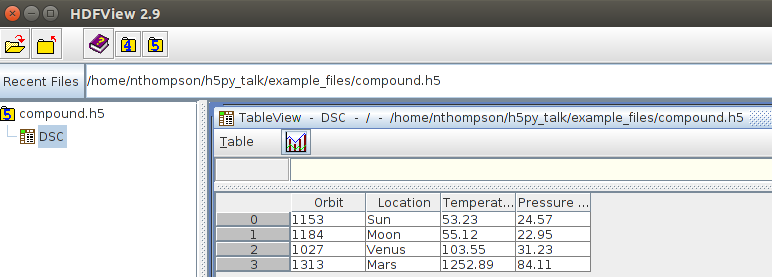
\includegraphics[scale=0.3]{fig/hdfview.png}
  \end{figure}
  \pause
  If you are attempting this in the Docker image, you'll need to set up X-window forwarding.
\end{frame}

\begin{frame}[fragile]
  \frametitle{Explore HDF5 Files}
  \begin{minted}{bash}
    $ h5ls example_files/compound.h5
    $ h5dump example_files/compound.h5
  \end{minted}
\end{frame}

\begin{frame}[fragile]
  \frametitle{New Visualization Tool:}
  \begin{minted}{bash}
    $ git clone https://github.com/HDFGroup/hdf-compass.git
    $ cd hdf-compass
    $ python HDFCompass.py
  \end{minted}
\end{frame}


\begin{frame}[fragile]
\frametitle{First HDF5 File}
\begin{minted}{python}
>>> import h5py
>>> import numpy as np
>>> f = h5py.File('stock_prices.hdf5')
v>>> f['/stock_prices/DJIA/MMM'] = np.random.random(2048)
>>> f['/stock_prices/DJIA/MMM'].attrs['sample_rate'] = 1
>>> f['/stock_prices/NASDAQ/MU'] = np.random.random(2048)
>>> f['/stock_prices/NASDAQ/MU'].attrs['sample_rate'] = 1
>>> f.close()
\end{minted}
\end{frame}

\begin{frame}[fragile]
  \frametitle{Analyzing HDF5 file}
  \begin{minted}{python}
    >>> import h5py
    >>> f = h5py.File('stock_prices.hdf5', 'r')
    >>> [key for key in f.keys() ]
    >>> ['stock_prices']
    >>> list(f.keys())
  \end{minted}
  \pause
  Use a callback to get more details:
  \begin{minted}{python}
    >>> def print_attrs(name, obj):
    >>>     print(list(obj))
    >>>     print(name)
    >>>
    >>> f.visititems(print_attrs)
    >>>
    >>> def p(name):
    >>>     print(name)
    >>>
    >>> f.visit(p)
  \end{minted}
\end{frame}

\begin{frame}[fragile]
  \frametitle{Within-Dataset Compression}
  Normally compressing data \emph{within} a file is unforgivable, but HDF5 makes it transparent:
  \begin{minted}{bash}
    >>> import h5py
    >>> import numpy
    >>> f = h5py.File('compressed.hdf5')
    >>> zipped_dst = f.create_dataset('ones',
                                      shape=(4096,), 
                                      dtype='int32',
                                      compression='gzip')
    >>> zipped_dst = np.ones(4096)
    >>> f.close()
    >>> g = h5py.File('compressed.hdf5', 'r')
    >>> dst = g['ones']
    >>> a = dst[:]
    >>> len(a)
    4096
    >>> a
    array([1, 1, 1, ..., 1, 1, 1], dtype=int32)
  \end{minted}
\end{frame}

\begin{frame}[fragile]
  \frametitle{Shuffle filters}
  You can't compress random data, but you can compress random data that is stored in a datatype that is larger than the range of random values:
  \begin{minted}{python}
    >>> f = h5py.File('compress_random.hdf5')
    >>> a = np.random.randint(low=0, high=256, size=10000)
    >>> f.create_dataset('rands', shape=(len(a),), data=a)
    >>> f.close()
  \end{minted}
  Now we can hexdump \texttt{compress\_random.hdf5} and see that all the entropy is in the first byte:
  \begin{minted}{bash}
    $ hexdump -v compress_random.hdf5
    0000e80 004d 0000 0000 0000 00a8 0000 0000 0000
    0000e90 00f5 0000 0000 0000 00d0 0000 0000 0000
    0000ea0 007e 0000 0000 0000 00bd 0000 0000 0000
    0000eb0 0075 0000 0000 0000 007b 0000 0000 0000
    0000ec0 0026 0000 0000 0000 0021 0000 0000 0000
    0000ed0 0027 0000 0000 0000 0048 0000 0000 0000
    0000ee0 0043 0000 0000 0000 0009 0000 0000 0000
    ...
  \end{minted}
\end{frame}

\begin{frame}[fragile]
  \frametitle{Shuffle Filters}
  We might get a better compression ratio if we move all the random bytes to one region on disk.

  In numpy this is called ``shuffling'', and can be achieved via:
  \begin{minted}{python}
    >>> f.create_dataset('rands',
                         shape=(len(a),),
                         data=a,
                         compression='gzip',
                         shuffle=True)
  \end{minted}
  In my test, gzip got a compression ratio of 3.86, and gzip+shuffle got a compression ratio of 5.79.    
\end{frame}

\begin{frame}[fragile]
  \frametitle{Checksumming}
  HDF5 has support for the Fletcher 32 checksum, which can be enabled via:
  \begin{minted}{python}
    >>> f.create_dataset('rands',
                        shape=(len(a),),
                        data=a,
                        fletcher32=True)
  \end{minted}
  If we use hexedit to alter this file and load the data, we get:
  \begin{minted}{python}
    >>> f = h5py.File('fletcher_checked.hdf5')
    >>> g = f['rands']
    >>> g[...]
    Traceback (most recent call last):
    OSError: Can't read data (Data error detected by fletcher32 checksum)
  \end{minted}
\end{frame}

\begin{frame}[fragile]
  \frametitle{h5repack}
  If you forgot to put checksumming, compression, or shuffling into your Python code during write, you can add it later with h5repack:
  \begin{minted}{bash}
    $ h5repack -v -f SHUF -f GZIP=9 -f FLET original.h5 copy.h5
  \end{minted}
\end{frame}

\begin{frame}[fragile]
  \frametitle{h5repack}
  h5repack also ``defragments'' your hdf5 file:
  \begin{minted}{python}
    >>> f = h5py.File('repack.hdf5')
    >>> a = np.random.rand(50000)
    >>> b = np.random.rand(35000)
    >>> c = np.random.rand(86000)
    >>> d = np.random.rand(87434)
    >>> f.create_dataset('a', shape=(len(a),), data=a)
    >>> f.create_dataset('b', shape=(len(b),), data=b)
    >>> f.create_dataset('c', shape=(len(c),), data=c)
    >>> f.create_dataset('d', shape=(len(d),), data=d)
    >>> f.flush()
    >>> del f['c']
    >>> f.flush()
    >>> f.close()
  \end{minted}
  This creates a file with a ``hole'' in it; now repack:
  \begin{minted}{bash}
    $ h5repack repack.hdf5 packed.hdf5
    ls -l repack.hdf5 packed.hdf5
    -rw-r--r-- 1 root root 1381616 Sep  4 16:35 packed.hdf5
    -rw-r--r-- 1 root root 2071664 Sep  4 16:34 repack.hdf5
  \end{minted}
  
\end{frame}


\begin{frame}[fragile]
  \frametitle{Fill-values}
  Arrays are filled with zeros by default, which is annoying:
  \begin{minted}{bash}
    >>> dset = f.create_dataset('waveform',
                                shape=(2048,),
                                dtype=np.float64,
                                fillvalue=np.nan)
    >>> dset[...]
    array([ nan,  nan,  nan, ...,  nan,  nan,  nan])
  \end{minted}
\end{frame}

\begin{frame}[fragile]
\frametitle{Chunked Storage}
Imagine that we are doing real-time monitoring; data is continuously appended to a dataset.

We don't know our uptime, so we need to tell HDF5 that our array is of arbitrary size
\begin{minted}{python}
>>> dset = f.create_dataset('trace', shape=(0, ), maxshape=(None,), chunks=(15000, ))
\end{minted}
The \texttt{maxshape=(None,)} makes the trace-length arbitrary

Why do we need \texttt{chunks=(15000,)} for arbitrary lengthed vectors?
\end{frame}


\begin{frame}[fragile]
  \frametitle{Chunked Storage}
  We can only resize chunked datasets:
  \begin{minted}{python}
    >>> dset = f.create_dataset('trace', shape=(0,))
    >>> dset.chunks
    ...
    >>> dset.resize((15000,))
        TypeError: Only chunked datasets can be resized
  \end{minted}
\end{frame}

\begin{frame}[fragile]
  \frametitle{Chunked Storage}
  Pseudo-code for real-time monitoring:
  \begin{minted}{python}
    dset = f.create_dataset('trace',
                  shape=(0, ),
                  maxshape=(None,),
                  chunks=(15000,),
                  fillvalue=np.nan)
    while True:
        trace_diff = np.random.rand(15000)
        l = len(dset)
        dset.resize((l+len(trace_diff),))
        dset[l:l+len(trace_diff)] = trace_diff
        time.sleep(60)
  \end{minted}
\end{frame}


\begin{frame}[fragile]
  \frametitle{Filter Pipelines}
  These options can be combined arbitrarily; the sequence of operations to read/write is then called a \emph{filter pipeline}:
  \begin{minted}{python}
    dset = f.create_dataset('trace',
                   shape=(0,),
                   maxshape=(None,),
                   chunks=(15000,),
                   fillvalue=np.nan,
                   compression='gzip',
                   shuffle=True,
                   fletcher32=True)
  \end{minted}
\end{frame}

\begin{frame}[fragile]
\frametitle{Compound Datatypes}
Sometimes we want to store a C-style struct in a HDF5 dataset; take for example shear velocity, compressional velocity and density from seismology. We don't want to decouple these datasets so we make a struct:
\begin{minted}{python}
comp_type = np.dtype([('compressional', 'f8'),
                      ('shear', 'f8'),
                      ('density', 'f8')])
data = np.empty(shape=(num,), dtype=comp_type)
for i in range(num):
    data[i] = (compressional[i], shear[i], rho[i])

dataset = np.create_dataset('rock_properties', (num,), comp_type)
dataset[...] = data
f.close()
\end{minted}
\end{frame}

\begin{frame}
  \frametitle{Real-time monitoring}
  HDF5 and h5py now have support for \emph{single-writer, multiple reader parallelism}, but there is some pain associated.

  You must use an experimental version of HDF5, and only on posix-compliant filesystems is it guaranteed to be race-free. (NFS is not posix-compliant).
  \begin{minted}{bash}
  $ cd v19
  $ docker build -t hdf5v19 .
  $ docker run -it -v `pwd`:/data hdf5v19 /bin/bash
  # cd data
  # ./writer.py &
  # ./reader.py &
  \end{minted}	
\end{frame}


\begin{frame}[fragile]
\frametitle{Compound Datatypes}
Some calculations only query compressional velocity, so we want to extract just that:
\begin{minted}{python}
>>> f = h5py.File('velocity.h5', 'r')
>>> g = f['rock_properties']
>>> p = g['compressional']
>>> p
array([ 3000.,  3000.,  3000., ...,  3000.,  3000.,  3000.])
\end{minted}
Putting part of a struct into a contiguous section of RAM this easily is huge.
\end{frame}

\begin{frame}[fragile]
\frametitle{Extensibility of Compound Datatypes}
Client code won't fail if I add another property to the compound datatype:
\begin{minted}{python}
comp_type = np.dtype([('compressional', 'f8'),
                      ('shear', 'f8'),
                      ('density', 'f8'),
                      ('Q', 'f8')])
data = np.empty(shape=(num,), dtype=comp_type) 
dataset = np.create_dataset('rock_properties', (num,), comp_type)
dataset[...] = data
\end{minted}
This doesn't obviate the need for versioning, but it makes it \emph{much easier}.
\end{frame}


\begin{frame}[fragile]
  \frametitle{Filesystem in a File: Hardlinks}
  You can create hardlinks within an HDF5 file:
  \begin{minted}{python}
    >>> import h5py
    >>> f = h5py.File('hardlink_example.hdf5', 'w')
    >>> g = f.create_group('x')
    >>> f['y'] = g
    >>> f['y'] == f['x']
    True
    >>> f.close()
  \end{minted}
  Not 100\% convinced of the utility of this . . . but it gets us thinking of HDF5 as a filesystem in a file. We can see links via h5ls:
  \begin{minted}{bash}
    $ h5ls -vlr hardlink_example.hdf5
    Opened ``hardlink_example.hdf5'' with sec2 driver.
    /                        Group
    Location:  1:96
    Links:     1
    /x                       Group
    Location:  1:800
    Links:     2
    /y                       Group, same as /x
  \end{minted}
\end{frame}

\end{document}
